\documentclass{beamer}
\usepackage[utf8]{inputenc}
\usepackage[spanish]{babel}
\usepackage{graphicx}
\usepackage{booktabs}
\usepackage{ragged2e}
\usepackage{xcolor}
\definecolor{LightGray}{gray}{0.975}
\definecolor{links}{HTML}{2A1B81}
%\usepackage[urlcolor=blue]{hyperref}
\hypersetup{colorlinks,linkcolor=,urlcolor=blue}

\usepackage{tikz}
\usetikzlibrary{arrows,shapes}

\usepackage{algorithm}
\usepackage{algorithmic}

\usepackage{minted}
\usepackage{xcolor}
\definecolor{LightGray}{gray}{0.975}

\usepackage{listings}

%\usetheme{Warsaw}
\usefonttheme{serif}

\title[Backup \& Restore]{Database Administration}
\subtitle{Lecture 07: Backup and Restore.}
\author{Valeja and Gonzales.}
\date{\today}

\setbeamertemplate{navigation symbols}{}%remove navigation symbols

\defbeamertemplate*{footline}{shadow theme}
{%
  \leavevmode%
  \hbox{\begin{beamercolorbox}[wd=.5\paperwidth,ht=2.5ex,dp=1.125ex,leftskip=.3cm plus1fil,rightskip=.3cm]{author in head/foot}%
    \usebeamerfont{author in head/foot} Database Administration \hfill \insertshorttitle
  \end{beamercolorbox}%
  \begin{beamercolorbox}[wd=.5\paperwidth,ht=2.5ex,dp=1.125ex,leftskip=.3cm,rightskip=.3cm plus1fil]{title in head/foot}%
    \usebeamerfont{title in head/foot} \hfill \insertframenumber\,/\,\inserttotalframenumber%
  \end{beamercolorbox}}%
  \vskip0pt%
}

\AtBeginSection[]
{
     \begin{frame}<beamer>
     \frametitle{Plan}
     \tableofcontents[currentsection]
     \end{frame}
}

\newcommand{\toRight}[1]{
    \begin{FlushRight}
        {\tiny #1}
    \end{FlushRight}
} % Align to right

\begin{document}

\frame{\titlepage}

\begin{frame}{Database Administration: Backup and Restore.}
    \centering
    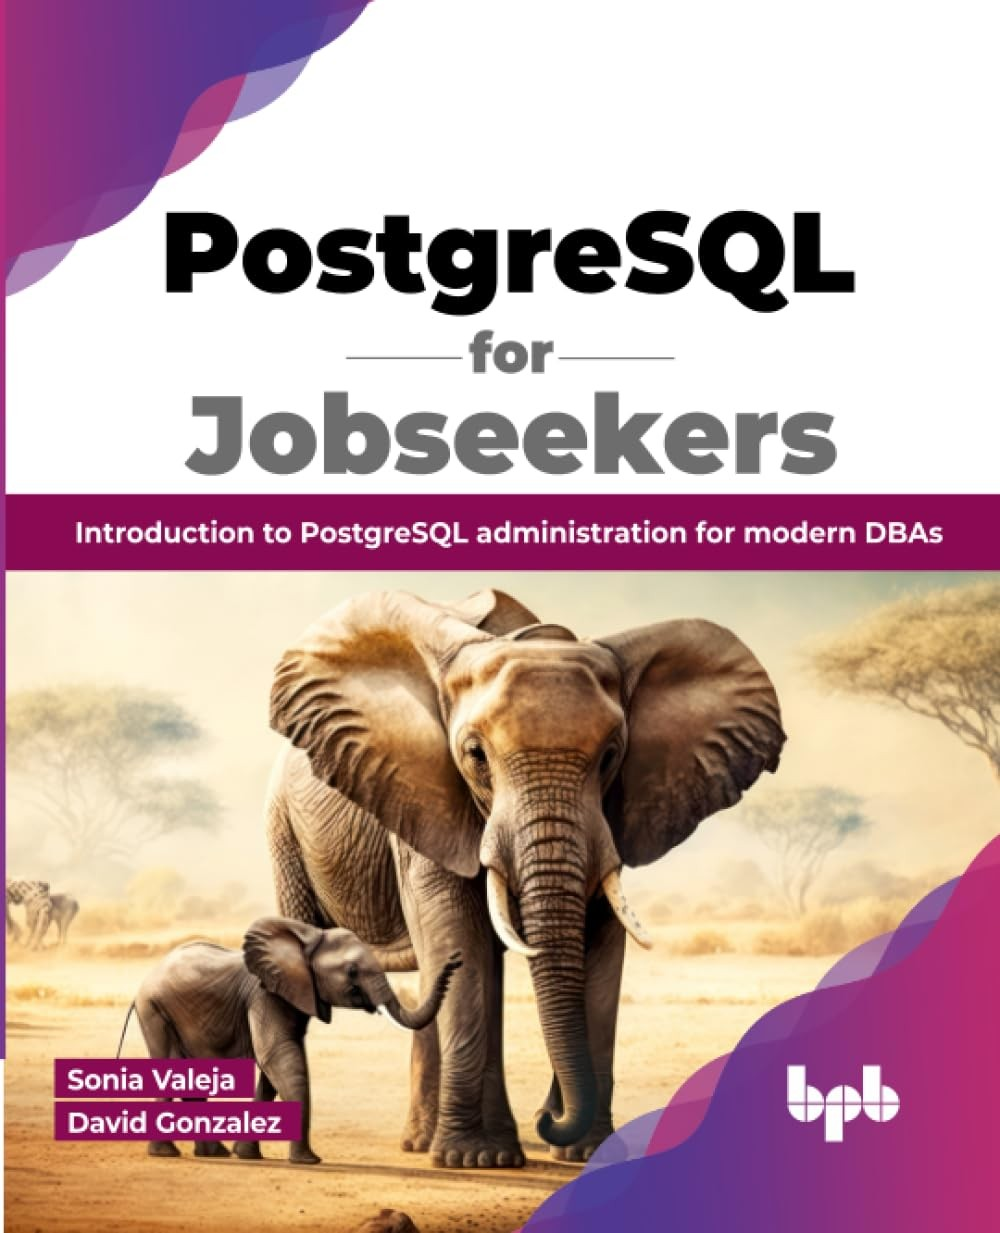
\includegraphics[width=0.4\textwidth]{figures/book_cover}\\
    \vspace{2mm}
    {
        \scriptsize
        Content has been extracted from \textit{PostgreSQL for Jobseekers (Chapter 7)}, by Sonia Valeja and David Gonzales, 2023.  Visit \url{https://bpbonline.com/products/postgresql-for-jobseekers}.\\
    }
\end{frame}

\begin{frame}{Introduction}
    \begin{itemize}
        \item Regular backups are crucial for database administration.
        \item Backups enable recovery from accidental changes.
        \item PostgreSQL provides multiple backup and restore tools.
    \end{itemize}
\end{frame}

\begin{frame}{Types of Backups}
    \begin{itemize}
        \item \textbf{Physical Backup}: Copies entire data directory.
        \item \textbf{Logical Backup}: Exports data in human-readable format.
    \end{itemize}
\end{frame}

\begin{frame}{Physical Backup}
    \begin{itemize}
        \item Uses filesystem-level copying.
        \item Steps:
        \begin{enumerate}
            \item Create a checkpoint.
            \item Copy data directory (e.g., using \texttt{tar} or \texttt{rsync}).
            \item Stop backup process.
        \end{enumerate}
        \item Example tool: \texttt{pg\_basebackup}.
    \end{itemize}
\end{frame}

\begin{frame}{Logical Backup}
    \begin{itemize}
        \item Exports data in SQL format.
        \item Allows individual table or database backups.
        \item Example tools:
        \begin{itemize}
            \item \texttt{pg\_dump} for single database.
            \item \texttt{pg\_dumpall} for full cluster backup.
        \end{itemize}
    \end{itemize}
\end{frame}

\begin{frame}{Restore Methods}
    \begin{itemize}
        \item \texttt{psql}: Restores backups in plain SQL format.
        \item \texttt{pg\_restore}: Restores backups from compressed/custom format.
    \end{itemize}
\end{frame}

\begin{frame}{Advanced Backup Tools}
    \textbf{pgBackRest}
    \begin{itemize}
        \item Supports full, incremental, and differential backups.
        \item Uses parallelism for faster operations.
        \item Supports cloud storage.
    \end{itemize}
\end{frame}

\begin{frame}{Barman}
    \begin{itemize}
        \item Used for remote backups.
        \item Provides incremental backup and deduplication.
        \item Maintains a backup catalog.
    \end{itemize}
\end{frame}

\begin{frame}{pg\_probackup}
    \begin{itemize}
        \item Provides incremental restore to save time.
        \item Supports backup merging and deduplication.
        \item Offers parallelism and remote operations.
    \end{itemize}
\end{frame}

\begin{frame}{Conclusion}
    \begin{itemize}
        \item PostgreSQL supports both physical and logical backups.
        \item Several tools exist to manage and automate backups.
        \item Choosing the right backup strategy depends on the use case.
    \end{itemize}
\end{frame}

\begin{frame}{Database Administration: Backup and Restore.}
    \centering
    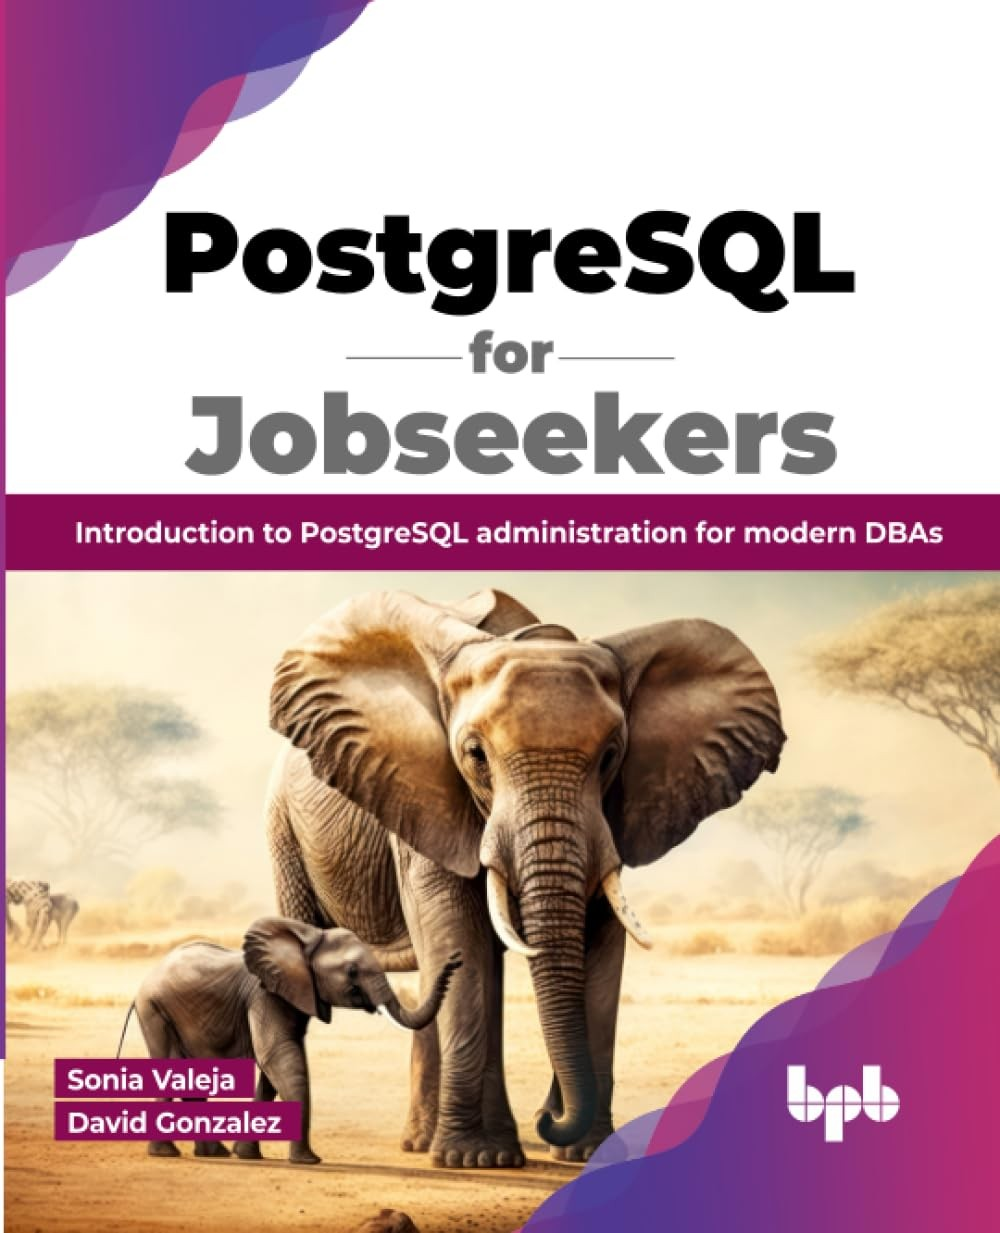
\includegraphics[width=0.4\textwidth]{figures/book_cover}\\
    \vspace{2mm}
    {
        \scriptsize
        Content has been extracted from \textit{PostgreSQL for Jobseekers (Chapter 7)}, by Sonia Valeja and David Gonzales, 2023.  Visit \url{https://bpbonline.com/products/postgresql-for-jobseekers}.\\
    }
\end{frame}

\end{document}
